\documentclass[a4paper, 12pt]{article}  		% classe du document

\usepackage[latin1]{inputenc} 		% packages english 
\usepackage[english]{babel}
\usepackage{url}
\usepackage{listings} 
\usepackage{color} 
\usepackage{multicol}

\definecolor{colKeys}{rgb}{0,0,1} 
\definecolor{colIdentifier}{rgb}{0,0,0} 
\definecolor{colComments}{rgb}{0,1,0} 
\definecolor{colString}{rgb}{0.6,0.1,0.1} 

\lstset{%configuration de listings 
float=hbp,% 
basicstyle=\ttfamily\small, % 
identifierstyle=\color{colIdentifier}, % 
keywordstyle=\color{colKeys}, % 
stringstyle=\color{colString}, % 
commentstyle=\color{colComments}, % 
columns=flexible, % 
tabsize=2, % 
frame=trBL, % 
frameround=tttt, % 
extendedchars=true, % 
showspaces=false, % 
showstringspaces=false, % 
numbers=left, % 
numberstyle=\tiny, % 
breaklines=true, % 
breakautoindent=true, % 
captionpos=b,% 
xrightmargin=0.8cm, % 
xleftmargin=0.8cm 
} 

%%%%%%%%%%%%%%%%%%%%%%%%%%%%%%%%%%%%%%%%%%%%%%%%%%

\usepackage[top=2.5cm, bottom=3cm, left=2.5cm, right=2.5cm]{geometry} 		% marges
\usepackage{setspace} 		% interligne

\usepackage{graphicx}  		% package figures
\usepackage{float}
\graphicspath{{images/}}

\usepackage{multirow}

\begin{document}	

\begin{titlepage}
\begin{center}
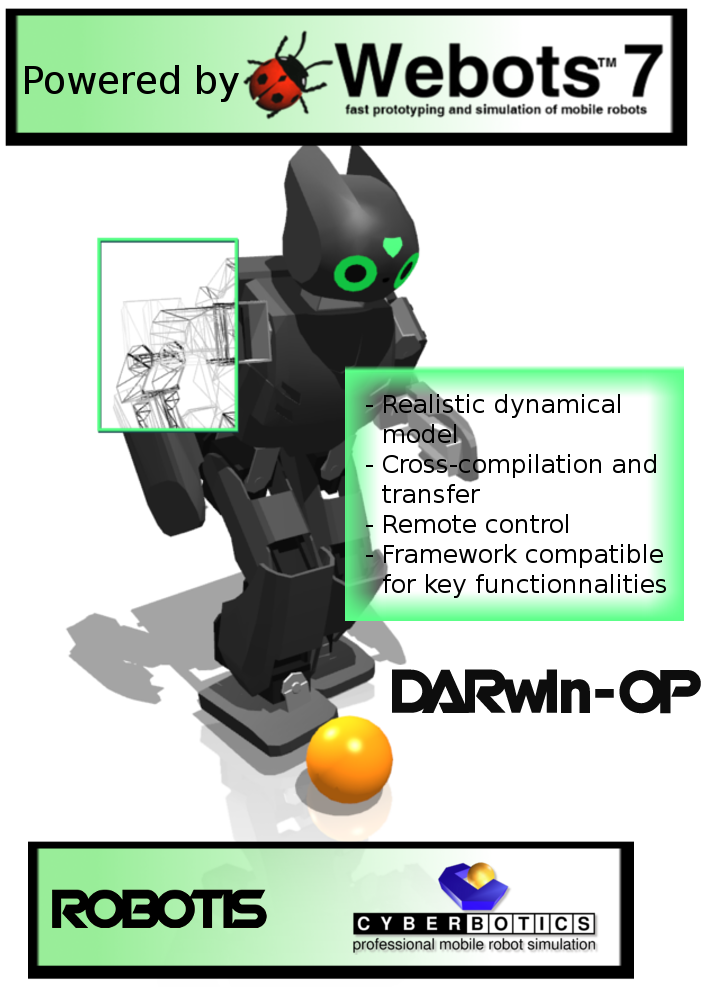
\includegraphics[width=17cm]{darwin-op.png}
\end{center}
\end{titlepage}


%%%%%%%%%%%%%%%%%%%%%%%%%%%%%%%%%%%%%%%%%%%%%%%%%%%%%%%%%%%%%%%%%%%%%%%%%%%%%%%%%


\newpage

\thispagestyle{empty}
\setcounter{page}{0}

\begin{center}
\vspace{5cm}
\Huge{DARwIn-OP with Webots User Guide}\\
\vspace{0.5cm}
\normalsize{release 1.0.0}\\

\vspace{3cm}
\LARGE{Copyright \copyright 2013 Cyberbotics Ltd.}\\
\vspace{0.5cm}
\large{All Rights Reserved}\\

\vspace{2cm}
\normalsize{\textbf{www.cyberbotics.com}}\\

\vspace{4cm}
\LARGE{Authors}\\
\vspace{0.5cm}
\normalsize{Fabien Rohrer}\\
\small{fabien.rohrer@cyberbotics.com}\\
\vspace{0.2cm}
\normalsize{\&}\\
\vspace{0.2cm}
\normalsize{David Mansolino}\\
\small{david.mansolino@epfl.ch}\\

\vspace{4cm}
\Large{\today}

\end{center}

% Abstract
\newpage
\thispagestyle{empty}
\setcounter{page}{0}

\renewcommand{\abstractname}{\huge{Foreword}}
\begin{abstract}
\vspace{3cm}
This document will explain you how is it possible to program the DARwIn-OP robot using Webots. Webots allows to program both the virtual robot model and the real robot by crosscompiling programs, or by remote-controlling the robot.\\

In the first chapters, all the features of the simulation model of the DARwIn-op will be presented and the examples included in Webots will be explained.\\

Then, in the following chapters, the possibilities of interaction with the real robot (real-time sensors viewing, cross-compilation and controller installation) will be explained.\\

We hope that you will enjoy working with Webots, and that it will greatly simplify your work with the DARwIn-OP.\\


\end{abstract}

%%%%%%%%%%%%%%%%%%%%%%%%%%%%%%%%%%%%%%%%%%%%%%%%%%%%%%%%%%%%%%%%%%%%%%%%%%%%%%%%%

\newpage
\thispagestyle{empty}
\setcounter{page}{0}

\begin{spacing}{0.9}
\tableofcontents
\thispagestyle{empty}
\end{spacing}

%%%%%%%%%%%%%%%%%%%%%%%%%%%%%%%%%%%%%%%%%%%%%%%%%%%%%%%%%%%%%%%%%%%%%%%%%%%%%%%%%

\newpage
\section{DARwIn-OP}
The Darwin-op is an open source miniature humanoid robot platform with advanced computational power. The name DARwIn-OP means Dynamic Anthropomorphic Robot with Intelligence-Open Platform. It is developed and manufactured by ROBOTIS (a Korean robot manufacturer) in collaboration with the University of Pennsylvania.\\

The DARwIn-OP is mainly used by universities and research centers for educational and research purpose. It has a total of 20 degrees of freedoms:
\begin{itemize}
\item 2 in the head.
\item 3 in each arm.
\item 6 in each leg.
\end{itemize}

This robot is available at a fairly low price and is based on open source components (both hardware and software). It has been used in the RoboCup international competition with some success.\\

The DARwIn-OP robot has been fully integrated into Webots in collaboration with ROBOTIS. By using DARwIn-OP in conjunction with Webots you will have the following benefits compared to the use of ROBOTIS API directly on the real robot:
\begin{description}
\item[Simulation ] You will be able to test your controller in simulation, without any risk of damaging the robot. You will also be able to run automatically a lot of different simulations in a very small amount of time (to tune up parameters for example), which would be impossible to do with the real robot.
\item[Cross compilation ] When your controller is doing fine in simulation, you will be able to send and run it on the real robot without changing anything to your code, just by pressing a button in the robot window.
\item[Remote control ] To debug or understand your controller's behavior, you will be able to see in real time the state of all the sensors and actuators on the computer screen. This is available both in simulation and on the real robot, and here again this is done in just one click. You will also be able to run your controller on the computer, but instead of sending commands to and reading sensor data from the simulated robot, it sends commands to and reads sensor data from the real robot.
\item[Ease of use ] Webots greatly simplifies the programming of the robot. Indeed, Webots API is simple to understand and to use and come with a complete documentation.
\end{description}

%%%%%%%%%%%%%%%%%%%%%%%%%%%%%%%%%%%%%%%%%%%%%%%%%%%%%%%%%%%%%%%%%%%%%%%%%%%%%%%%%%

\newpage
\section{Simulation model}

The simulation model of DARwIn-OP was design to be as close as possible to the real one. It is equiped with the following sensors and actuators :
\begin{itemize}
\item 20 servos
\item 5 LEDs (including 2 RGB ones)
\item A 3 axes accelerometer
\item A 3 axes gyroscope
\item A camera
\end{itemize}

The accelerometer returns values between 0 and 1024 corresponding to values between -3 [g] to +3 [g] like on the real robot. For the gyro, it returns also values between 0 and 1024, corresponding to values between -1600 [deg/sec] and +1600 [deg/sec], here again similarly to the values returned by the real robot. Their respective names are \textit{Accelerometer} and \textit{Gyro}.

The camera is a RGBA camera and has a basic resolution of 160x120 pixels, but it can be changed to any value. The horizontal field of view is 1.0123 [rad].\\

Each of the 2 RBG LEDs, called \textit{HeadLed} and \textit{EyeLed}, is split in two separated parts, one on the head of the robot and one other small part on the back panel of the robot. There are also three other standard LEDs on the back panel of the robot, they are called \textit{BackLedGreen}, \textit{BackLedBlue} and \textit{BackLedRed}.\\

The name of the 20 servos are the following :

\begin{table}[H]
\begin{center}
\begin{tabular}{ | c | c | c | c | c | c | c | c |  }
\hline
ID & Name & ID & Name & ID & Name & ID & Name\\ 
\hline
\hline
1 & ShoulderR & 2 & ShoulderL & 3 & ArmUpperR & 4 & ArmUpperL \\
\hline
5 & ArmLowerR & 6 & ArmLowerL & 7 & PelvYR & 8 & PelvYL \\
\hline
9 & PelvR & 10 & PelvL & 11 & LegUpperR & 12 & LegUpperL \\
\hline
13 & LegLowerR & 14 & LegLowerL & 15 & AnkleR & 16 & AnkleL \\
\hline
17 & FootR & 18 & FootL & 19 & Neck & 20 & Head \\
\hline
\end{tabular}
%\caption{...}
\label{tab::servosName}
\end{center}
\end{table}

The corresponding position of each servo can be seen in figure \ref{Actuator}.\\
Each of the 20 servos has the following configuration:
\begin{table}[H]
\begin{center}
\begin{tabular}{ | c | c | c | }
\hline
maxForce & 2.5 & $N*m$ \\ 
\hline
acceleration & 55 & $rad/s^{2}$ \\ 
\hline
maxVelocity & 12.26 & $rad/s$ \\ 
\hline
dampingConstant & 0.002 & $ $ \\ 
\hline
staticFriction & 0.025 & $N*m$ \\ 
\hline
\end{tabular}
%\caption{...}
\label{tab::servosConfig}
\end{center}
\end{table}


\newpage
\vspace{5cm}
\begin{figure}[H]
\begin{center}
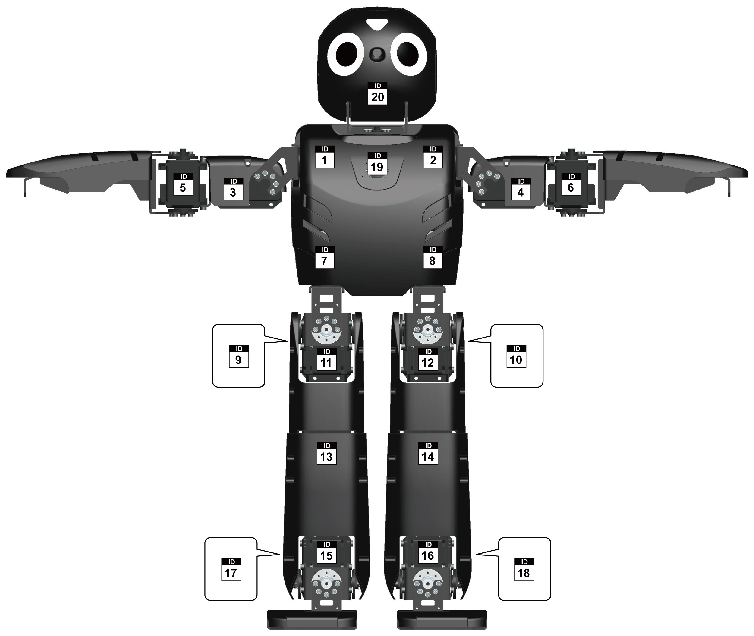
\includegraphics[width=16cm]{DARwIn-OP_Actuator.png}
\caption{Position of the servos}
\label{Actuator}
\end{center}
\end{figure}
For more information on the use of all of these sensors/actuators refer to the \textit{Reference Manual} of Webots \,\footnote{ Reference Manual available at: \url{http://www.cyberbotics.com/reference/}}.\\



\newpage
The physical model is very realistic and self collision check is available. To activate the self collision expand DARwIn-OP in the scene tree and set selfCollision field to true (see figure \ref{selfCollision}). Use the self collision check only if you need it, because it is very computationally costly and can therefore significantly slow down the simulation speed.\\

\begin{figure}[H]
\begin{center}
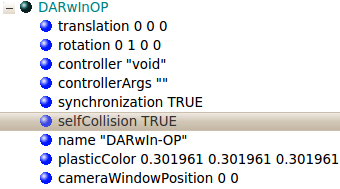
\includegraphics[width=8cm]{selfCollision.png}
\caption{Scene tree of the DARwIn-OP.}
\label{selfCollision}
\end{center}
\end{figure}

The following sensors/actuators are not present on the simulation model :
\begin{itemize}
\item The three buttons on the back of the robot are not present because they have no interest in the simulation.
\item The microphones are not present in simulation because sound is not yet supported in Webots.
\item The speakers are not present too because sound is not yet supported in Webots, but this will certainly be added soon. 
\end{itemize}

%%%%%%%%%%%%%%%%%%%%%%%%%%%%%%%%%%%%%%%%%%%%%%%%%%%%%%%%%%%%%%%%%%%%%%%%%%%%%%%%%%

\newpage
\section{Managers}

A library is provided in order to implement all the key functionalities of Robotis Framework in simulation. This library is divided in three parts called managers. Each manager implements a module of the Framework. The first one called \textit{Gait} manager allows you to use the walking algorithm of the Robotis Framework. The second one called \textit{Motion} manager allows you to play predefined motions stored in the \textit{motion\_4096.bin} file. The last one called \textit{Vision} manager, contains some image processing tools, useful for example to find a colored ball in the camera image.\\

\subsection{Gait Manager}
This manager implements the \textit{DARwInOPGaitManager} class and allows you to use the walking algorithm of the Framework.\\

A lot of parameters are available in the Framework algorithm to tune the gait. But in order to make this manager easy to use, only a subset of the parameters can be set. The other parameters are set to default values that are known to works fine. It is however possible to change them if needed, by changing the default values that are stored in a \textit{*.ini} configuration file. In appendix \ref{sec:walkParameter}, all the parameters of the gait are explained. The C++ constructor of DARwInOPGaitManager object is the following :\\

\lstset{language=c++} 
\lstset{commentstyle=\textit} 
\begin{lstlisting} 
DARwInOPGaitManager(webots::Robot *robot, const std::string &iniFilename);
\end{lstlisting}

The first parameter is the robot on which the algorithm applies and the second is the file name in which the default parameters are stored. The following method are available in order to modify the main parameters in your controller :\\

\lstset{language=c++} 
\lstset{commentstyle=\textit} 
\begin{lstlisting} 
void setXAmplitude(double x);
void setYAmplitude(double y);
void setAAmplitude(double a);
void setMoveAimOn(bool q);
void setBalanceEnable(bool q);
\end{lstlisting}

These are the open parameters, they have the following impact on the gait:\\
\begin{itemize}
\item X influences the length of the foot step forward, it can take any value between -1 and 1.
\item Y influences the length of the foot step in the side direction, it can take any value between -1 and 1.
\item A influences the angle of the gait and allows also the robot to rotate during the walk, it can take any value between 0 and 1.
\item If MoveAimOn is set, it allows the robot to rotate around something by inversing the sense of rotation, it can be very useful to turn around a ball in order to kick it in the right direction for example.
\item If BalanceEnable is set, the gyroscope is used in the control loop to make the walking gait more robust.
\end{itemize}

Finally the following method can be used in order to run the algorithm:\\
\lstset{language=c++} 
\lstset{commentstyle=\textit} 
\begin{lstlisting} 
void start();
void step(int ms);
void stop();
\end{lstlisting}
Start and stop need to be used to stop/start the algorithm and step is used to run \textit{ms} milliseconds of the algorithm.\\

Note that, in order to run, the gait manager needs to know the position of each servo and the values of the gyro. It is therefore essential to enable the gyro and the position feedback of each servo before to use it, if it is not the case, a warning will appear and they will automatically be enabled.\\

\subsection{Motion Manager}
This manager implement the \textit{DARwInOPMotionManager} class and allows you to play a predefined motion stored in the \textit{motion\_4096.bin} file. The main motions and their corresponding ids are listed in appendix \ref{sec:Motions}.\\

It is also possible to add custom motions to this file by using the \textit{Action Editor} tool \,\footnote{ More informations about this tool provided by ROBOTIS is available at: \url{www.support.robotis.com/ko/product/darwin-op/development/tools/action_editor.htm}}.\\

The constructor of \textit{DARwInOPMotionManager} object is the following :\\
\lstset{language=c++} 
\lstset{commentstyle=\textit} 
\begin{lstlisting} 
DARwInOPMotionManager(webots::Robot *robot);
\end{lstlisting}

It only needs a pointer to the robot to which it applies. Then, the following method can be used to play a motion:\\

\lstset{language=c++} 
\lstset{commentstyle=\textit} 
\begin{lstlisting} 
void playPage(int id);
\end{lstlisting}

This method only needs the id of the motion to be played.\\

\subsubsection{Motion Manager in mode step-by-step}

By default when starting a motion, the motion is run synchronously. That is the controller is stopped until the motion is finished. But it is also possible to run a motion asynchronously, in that case, the motion is started but the execution flow of the controller is not stopped. This can be done by calling the method \textit{playPage} with the second parameter set to false:\\
\lstset{language=c++} 
\lstset{commentstyle=\textit} 
\begin{lstlisting} 
void playPage(int id, bool sync = true);
\end{lstlisting}

This will initiate the motion, but not run it, then in order to play ms second of the motion, the following method need to be called (before the robot step):\\
\lstset{language=c++} 
\lstset{commentstyle=\textit} 
\begin{lstlisting} 
void step(int ms);
\end{lstlisting}

In order to know if the motion is finished, the following method can be called:\\
\lstset{language=c++} 
\lstset{commentstyle=\textit} 
\begin{lstlisting} 
bool isMotionPlaying();
\end{lstlisting}

A typical use of the motion manager in mode step-by-step will be the following:\\
\lstset{language=c++} 
\lstset{commentstyle=\textit} 
\begin{lstlisting} 
mMotionManager->playPage(1, false);
while(mMotionManager->isMotionPlaying()) {
  mMotionManager->step(mTimeStep);
  /*
   * Do something,
   * like image processing for example
   */
  myStep();
}
\end{lstlisting}

\newpage
\subsection{Vision Manager}
This manager implement the \textit{DARwInOPVisionManager} class. The constructor of this class is the following :\\

\lstset{language=c++} 
\lstset{commentstyle=\textit} 
\begin{lstlisting} 
DARwInOPVisionManager(int width, int height, int hue, int hueTolerance, int minSaturation, int minValue, int minPercent, int maxPercent);
\end{lstlisting}
The parameters are the following : \\
\begin{itemize}
\item The widht of the image
\item The height of the image
\item The color hue of the target object to find
\item The tolerance on the color hue of the target object to find
\item The minimum color saturation of the target object to find
\item The minimum color value of the target object to find
\item The minimum percentage of color value in the image to validate the result
\item The maximum percentage of color value in the image to validate the result
\end{itemize}

To find the color hue of the target object and to understand the impact of the saturation and value you can refer to figure \ref{HSV}, for more information you can also find a lot of great documentation on the Internet about HSV colorspace.\\ 
\begin{figure}[H]
\begin{center}
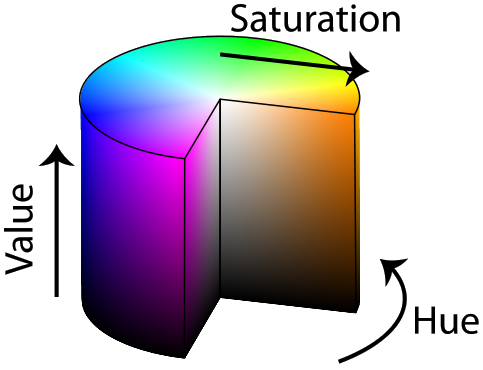
\includegraphics[width=6cm]{HSV.png}
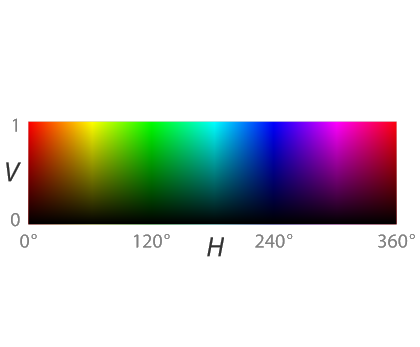
\includegraphics[width=6cm]{HV.png}
\caption{HSV colorspace}
\label{HSV}
\end{center}
\end{figure}

\newpage
When an instance of this class is created, the \textit{getBallCenter} method can be used to find the position of the target object:\\

\lstset{language=c++} 
\lstset{commentstyle=\textit} 
\begin{lstlisting} 
bool getBallCenter(double &x, double &y, const unsigned char * image);
\end{lstlisting}
 
This method returns true if the target was found, and false otherwise. If found, the x and y variables are set. The image pointer indicates the original image buffer. In order to find the position of the target object, this method proceeds to the following steps:\\
\begin{itemize}
\item Store the BGRA version of the image in a buffer
\item Use this buffer to convert the image to HSV format
\item Use the \textit{Finder} class of the Framework to find the target object
\item Extract and save the position of the target object
\end{itemize}

Once this method was called it is possible to know which pixels of the image are part of the target object by using this function:\\

\lstset{language=c++} 
\lstset{commentstyle=\textit} 
\begin{lstlisting} 
bool isDetected(int x, int y);
\end{lstlisting}

This method returns true if the pixel (x,y) is part of the target object and false otherwise.\\


%%%%%%%%%%%%%%%%%%%%%%%%%%%%%%%%%%%%%%%%%%%%%%%%%%%%%%%%%%%%%%%%%%%%%%%%%%%%%%%%%%

\newpage
\section{Examples}

In this part we will see all the examples provided with Webots for the DARwIn-OP model. We will describe how they work, how to use them and what can be done with them. All the examples can be found in WEBOTS\_HOME/projects/robots/darwin-op/worlds.\\

The following buttons are the main ones used to control the simulation (they all are situated on top of the 3D view):
\begin{table}[H]
\begin{center}
\begin{tabular}{ c l }

\includegraphics{button_open.png} & \textbf{Open world} is used to open another example. \\

\includegraphics{button_revert.png} & \textbf{Revert} is used to reload the example file and restart the simulation. \\

\includegraphics{button_play.png} & \textbf{Run} is used to start the simulation at real time speed. \\

\includegraphics{button_stop.png} & \textbf{Stop} is used to stop the simulation. \\
\end{tabular}
\end{center}
\end{table}

You will also need to use the following buttons to edit the examples (they are situated on top of the text editor):
\begin{table}[H]
\begin{center}
\begin{tabular}{ c l }

\includegraphics{button_open.png} & \textbf{Open file} is used to open a new file in the text editor. \\

\includegraphics{button_save.png} & \textbf{Save file} is used to save the current file. \\

\includegraphics{button_compile.png} & \textbf{Build} is used to build the current project. \\

\includegraphics{button_clean.png} & \textbf{Clean} is used to clean all the compilation files of the current project. \\
\end{tabular}
\end{center}
\end{table}

You can find more information about the user interface in the corresponding chapter of the \textit{User Guide}\,\footnote{User Guide available at: \url{www.cyberbotics.com/guide}}.

\newpage
\subsection{Symmetry}

This example is very basic and explains the use of the servos.\\

\begin{figure}[H]
\begin{center}
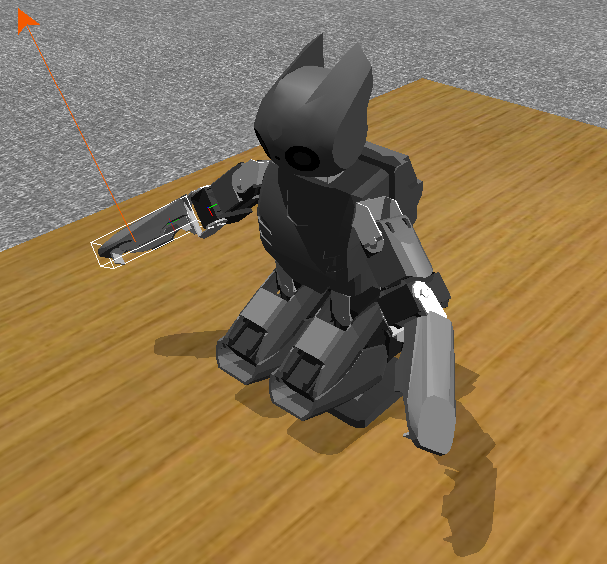
\includegraphics[width=10cm]{example_symmetry.png}
%\caption{...}
\label{example_symmetry.png}
\end{center}
\end{figure}

It starts by setting the motor force of the three servos of the right arm to zero in order to completely release this arm.
Then, in an infinite loop, the position of the previous three servos is read and displayed.
Finally, still in the loop, the opposite position of each servo of the right arm is applied to the corresponding servo of the left arm in order to mimic the motion of the right arm.\\
In order to move the right arm which is free in simulation, select the robot, then press Ctrl+Alt and left click on the arm, then without releasing the left button move the mouse. This will apply a force (symbolized by an arrow) which will make the arm move.\\
Note that it is very important to activate the position feedback of the servos in order to read their position. In this example, this is done in the constructor.\\

You can also try to add an oscillation of the head, by adding this in your main loop:
\lstset{language=c++} 
\lstset{commentstyle=\textit} 
\begin{lstlisting} 
mServos[18]->setPosition(sin(getTime()));
\end{lstlisting}

Then save the file, press the build button and finally revert the simulation to start the new controller.\\

This example is well suited for the cross-compilation and we recommended that you start by testing the cross-compilation tool by using this example.\\

\newpage
\subsection{VisualTracking}

This example illustrates the use of the camera (including the vision manager) and of the RGB LEDs.\\

\begin{figure}[H]
\begin{center}
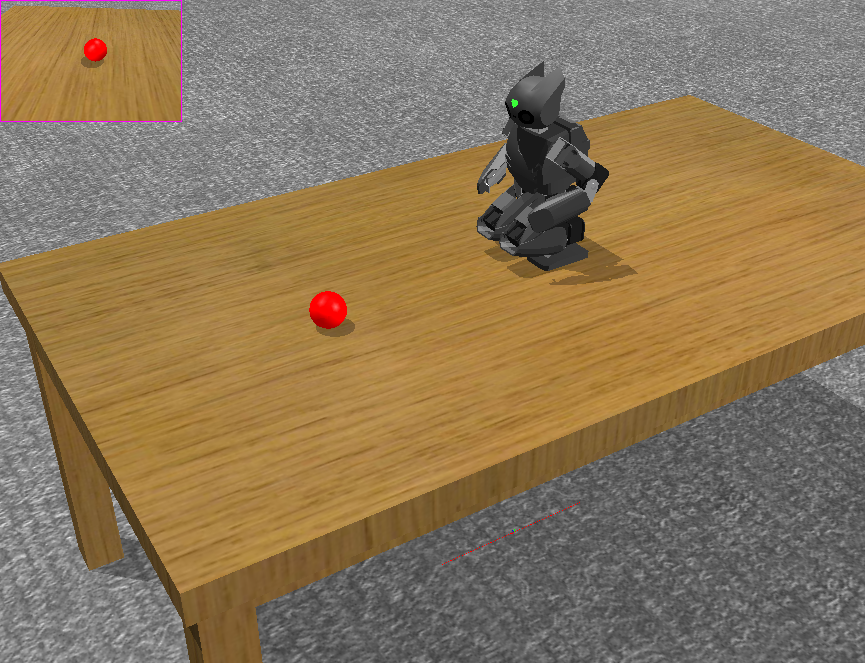
\includegraphics[width=10cm]{example_visualTracking.png}
%\caption{...}
\label{example_visualTracking.png}
\end{center}
\end{figure}

In the infinite loop the vision manager is used to find the red ball. 
Then, if the ball has been found the head led is set to green and otherwise to red.
Then, again, if the ball has been found the position of the two servos of the head is corrected to watch in the direction of the ball. To move the ball in simulation, press Ctrl+Shift and move the ball with the left button of the mouse pressed on it.\\

Try to change the color of the LED by changing this line :
\lstset{language=c++} 
\lstset{commentstyle=\textit} 
\begin{lstlisting} 
mHeadLED->set(0xFF0000);
\end{lstlisting}
Here the color is set in hexadecimal. The format is R8G8B8: The most significant 8 bits (left hand side) indicate the red level (between 0x00 and 0xFF). Bits 8 to 15 indicate the green level and the least significant 8 bits (right hand side) indicate the blue level. For example, 0xFF0000 is red, 0x00FF00 is green, 0x0000FF is blue, 0xFFFF00 is yellow, etc.\\

Try also to use the other RGB LED, this is done simply be exchanging \textit{mHeadLED} by \textit{mEyeLED}.\\

Here again this example is well suited for cross-compilation. You can adjust the color of the ball by changing the value in the constructor of DARwInOPVisionManager if your ball has a different color.\\

This example can also be used as a tool to tune the parameters of the vision manager in order to fit your application.\\


\newpage
\subsection{Walk}

This example illustrates the use of the gait and motion manager, the use of the keyboard, and also the use of the accelerometer.\\

\begin{figure}[H]
\begin{center}
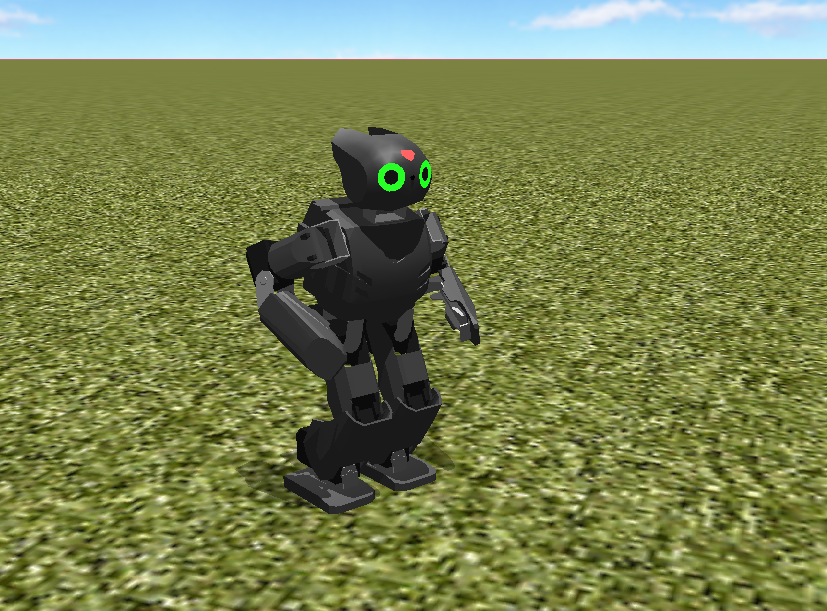
\includegraphics[width=10cm]{example_walk.png}
%\caption{...}
\label{example_walk.png}
\end{center}
\end{figure}

At the beginning of the controller, the motion manager is used to make the robot stand up, then the controller enters an infinite loop.
The first thing done in the loop is to check if the robot has not fallen down, this is achieved by using the accelerometer. Then if the robot has fallen down, the motion manager is used to make the robot to stand up. 
Then, the keyboard is read, if the space bar is pressed the robot start/stop to walk.
Then, the keys up/down/right/left are pressed to make the robot turn and move forward/backward, several keys can be pressed at the same time.\\

Try to add some more action by using more keys. You can for example use the \textit{KEYBOARD\_NUMPAD\_LEFT} and \textit{KEYBOARD\_NUMPAD\_RIGHT} keys to make a left/right shoot (page 13 and 12 in motion manager). You can also use normal keys like 'A' instead if you prefer.\\

You can also use another key to make the robot walk quicker or slower (change the XAmplitude sent to the gait manager, values must be between -1 and 1).\\

This example works in cross-compilation but you will need to connect a USB keyboard to the robot. Otherwise, it is recommended to test this example with the remote control in order to use the computer's keyboard instead.\\

This example can also be used to explore and test all the parameters of the gait.\\

\newpage
\subsection{Soccer}

This is a very complete example which used the three managers and almost all of the sensors.\\

\begin{figure}[H]
\begin{center}
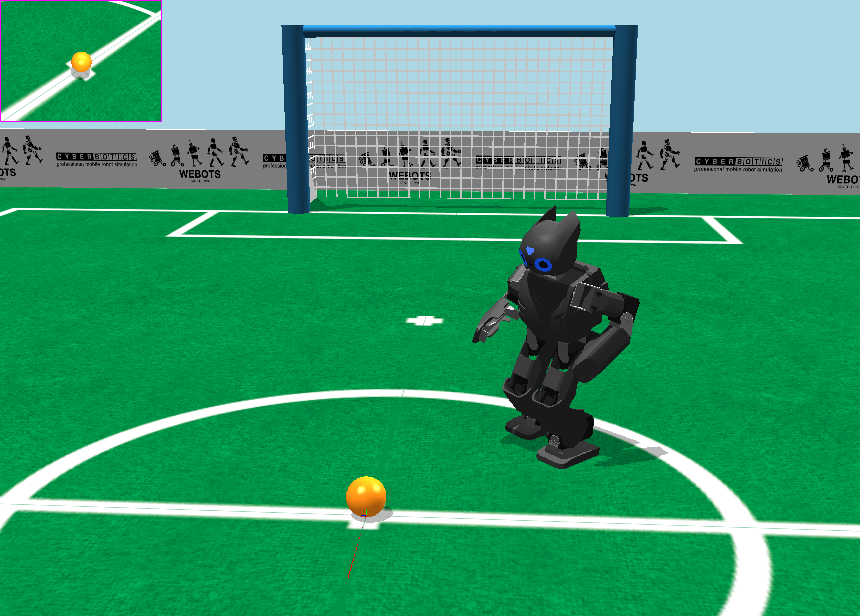
\includegraphics[width=10cm]{example_sample.png}
%\caption{...}
\label{example_sample.png}
\end{center}
\end{figure}

The controller is a very simple soccer player. It relies on most of the tools used in the previous example. We recommend you to study it by yourself and of course to improve it.\\

To extend this controller you can add new files to the project, but do not forget to also add them to the makefile (add the cpp files to the \textit{CXX\_SOURCES} section). This example is also a good starting point for developing a more complicated controller.\\

This example works in cross-compilation. But we recommend you to test it on a soft ground and away from any source of danger (stairs, hot surface, etc.), because the robot will move a lot and it is not excluded that it falls down from time to time.\\


%%%%%%%%%%%%%%%%%%%%%%%%%%%%%%%%%%%%%%%%%%%%%%%%%%%%%%%%%%%%%%%%%%%%%%%%%%%%%%%%%

\newpage
\section{Robot Window}

When you double click on the robot, a new window appears. This window is called \textit{Robot Window}, it has severals tabs allowing you to perform different things. The first four tabs concerns the simulation and remote control. They will be describe here, the last tab is used to interact with the real robot and will therefore be describe in the next sections.\\

In the unlikely case of something going wrong with the \textit{Robot Window} (freeze, bad behavior, etc.) you can at any time restart it by pressing the revert button of the simulation.\\

\paragraph*{Accelerometers} 
This tab can be used to investigate the values of the accelerometer while the controller is running. If the checkbox is checked, the values of the accelerometer are shown and plotted on the graph in real time. Four different types of graph can be plot. The first three are one axis in function of an other, and the last one, plots the value of the three axes in function of the time. The corresponding colors are the following:\\
\begin{itemize}
\item Red for axis X
\item Green for axis Y
\item Blue for axis Z
\end{itemize}

\begin{figure}[H]
\begin{center}
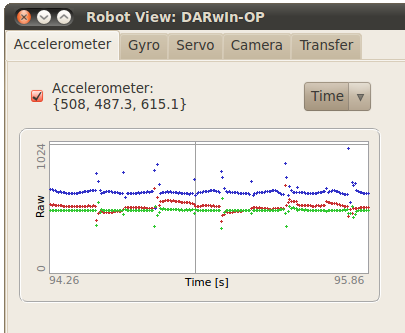
\includegraphics[width=10cm]{window_accel.png}
\label{window_accel}
\end{center}
\end{figure}

You can click any time on the graph to adjust the scale of the data currently plotted.\\

\newpage
\paragraph*{Cameras}
This tab is very simple, if the checkbox is checked, the picture of the camera is shown and updated in real time.\\

\begin{figure}[H]
\begin{center}
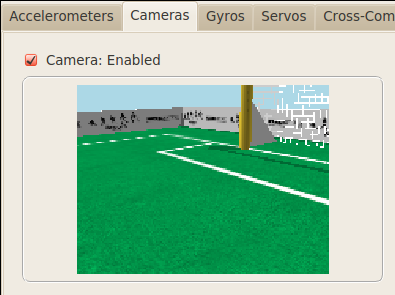
\includegraphics[width=10cm]{window_camera.png}
\label{window_camera}
\end{center}
\end{figure}

\paragraph*{Gyro}
This tab is very similar to the accelerometer tab but addresses the gyro. If the checkbox is checked, the values of the gyro are shown and plotted on the graph in real time. Here again four different types of graph can be plot. \\

\begin{figure}[H]
\begin{center}
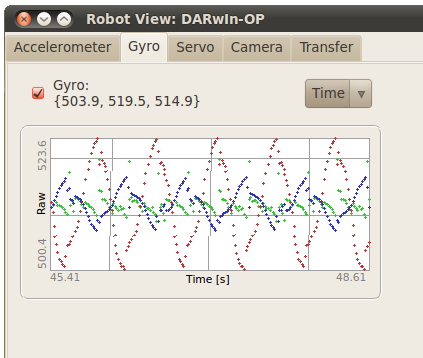
\includegraphics[width=10cm]{window_gyro.png}
\label{window_gyro}
\end{center}
\end{figure}

\newpage
\paragraph*{Servos}
Finally, this last tab can be used to see and influence the state of each servo. The use of each servo in the robot window can separately be set by checking/unchecking the corresponding checkbox of the servo. If the checkbox is checked, the value of the servo is shown and plotted in function of the time. On the graph, two different colors are used to distinguish the target value (in red) and the real value (in black). It is also possible to manually change the value of the servo by using the slider beside the graph.\\

\begin{figure}[H]
\begin{center}
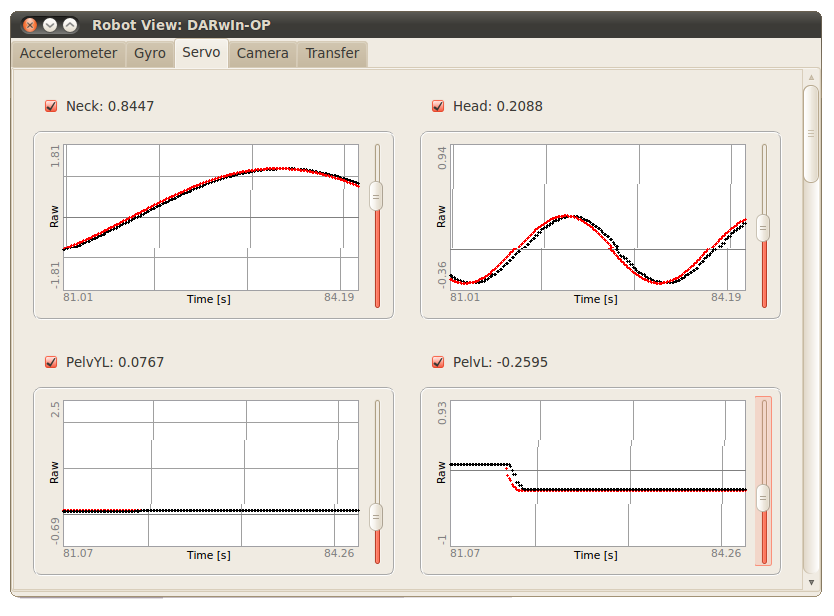
\includegraphics[width=14cm]{window_servos.png}
\label{window_servos}
\end{center}
\end{figure}


%%%%%%%%%%%%%%%%%%%%%%%%%%%%%%%%%%%%%%%%%%%%%%%%%%%%%%%%%%%%%%%%%%%%%%%%%%%%%%%%%

\newpage
\section{Cross-compilation}

To send your controller to the real robot and make it run on it, go to the \textit{Transfer} tab of the robot window (figure \ref{window_cross}).

\begin{figure}[H]
\begin{center}
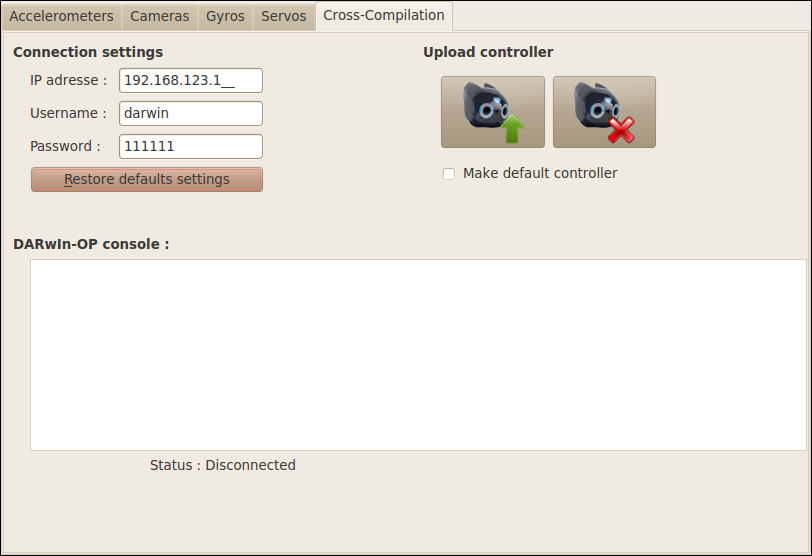
\includegraphics[width=13cm]{window_cross.png}
\caption{Transfer tab of the robot window.}
\label{window_cross}
\end{center}
\end{figure}

The first thing to do is to set the connections settings. The first setting is the IP address of the robot. If you use an Ethernet cable to connect to the robot, the IP address is 192.168.123.1. But if you use a wifi connection with the robot the address is not fixed, to know it, execute the \textit{ifconfig} command on the robot, the IP address is the \textit{inet addr} of wlan0 (warning, the address can sometimes change without any specific reason). The second parameter is the username with which you log-on on the robot, if you do not have explicitly changed it, the username is \textit{darwin}. Finally the last parameter is the password corresponding to the username, here again, if you do not have explicitly changed it, the password is \textit{111111}. Each time you connect successfully to the robot, all the settings are saved so that it is not necessary to set them each time you start the program. If you want to restore the default parameters of the connection, just click on the \textit{Restore default settings} button (Alt+r).\\

Before you can send your controller to the real robot you have to change the Makefile.darwin-op file to suit to your project. If you have added new files to the project, do not forget to add them to the \textit{CXX\_SOURCES} and if you have changed the project name, change also the \textit{TARGET} value.\\

\newpage
Before to send the controller you will also need to complete the \textit{Robot Config} section of the \textit{config.ini} file. You have two parameters to fill in:
\begin{description}
\item[Time step] The time step in milliseconds must be specified in the field \textit{time\_step}, a minimal time step of 16ms is requested, if no time step (or a time step smaller than 16ms) is set, the default time step of 16ms is used. Warning: Depending on the complexity of you controller, a time step of 16ms can not always be respected. For example using the camera or the manager can slow done the speed, so enable them only if you really need them.\\
\item[Camera resolution] The horizontal and vertical resolution of the camera must be set in the fields \textit{camera\_width} and \textit{camera\_height}. Only the resolutions specified in table \ref{tab:cameraResolution} are supported, if another resolution is set, the default resolution of 320x240 will be used.\\
\end{description}

\begin{table}[H]
\begin{center}
\begin{tabular}{ | c | c | c | }

\hline
Width [pixel] & Height [pixel] & FPS \\ 
\hline
\hline
320 & 240 & 30 \\
\hline
640 & 360 & 30 \\
\hline
640 & 400 & 30 \\
\hline
640 & 480 & 30 \\
\hline
768 & 480 & 28 \\
\hline
800 & 600 & 22.5 \\
\hline
\end{tabular}
\caption{Camera resolutions supported by the camera of the DARwIn-OP.}
\label{tab:cameraResolution}
\end{center}
\end{table}

\subsection{Send a controller to the robot}
To test your controller on the real robot press the following button :
\begin{figure}[H]
\begin{center}

\includegraphics[width=2.5cm]{send.png}
\label{send}
\end{center}
\end{figure}

Webots will then connect to the robot, if any error appears during the connection, the reason will be shown. If it is the first time you connect the robot with Webots, Webots will install all the files needed on the robot. This can take some time and some step are longer than other, so be patient please, this happens only on the first connection, the next ones will be shorter. You can also see in real time what is appening in the \textit{DARwIn-OP console}. Webots will also stop the auto start of the demo program at the startup of the robot, but don't worry the program is not suppressed and the auto start can easily be reinstalled (explanation follows).\\


Then the controller code itself is send to the robot. All the directory of the controller is send to the robot, so please put all the files needed by your controller in the same directory. The controller itself is then compiled for the robot and you can see the compilation in the \textit{DARwIn-OP console}. If the compilation success and the robot is close to the start position (figure \ref{start_position}) the controller will be initialized (head and eyes LED in red) and then started (head and eyes LED in green).\\

\begin{figure}[H]
\begin{center}
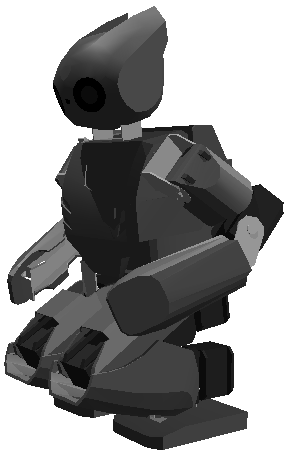
\includegraphics[width=5cm]{start_position.png}
\caption{Start position of the robot. The robot is sit down (same start position that in simulation).}
\label{start_position}
\end{center}
\end{figure}

It is recommended when testing a new controller whose behavior is not very certain to hold the robot by its handle.\\

To stop the controller press the following button :
\begin{figure}[H]
\begin{center}
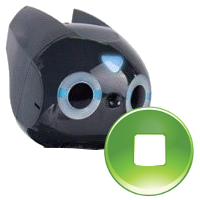
\includegraphics[width=2.5cm]{stop.png}
\caption{Stop button.}
\label{stop}
\end{center}
\end{figure}

This will stop the controller and clean all files previously sent to the robot.\\

You can also stop the controller by pressing the right button at the back of the robot. This will not entirely stop the controller but will at least avoid the robot from moving. It will also release the torque of all the servos.\\

\subsection{Permanently install a controller to the robot}
If you want to install the controller on the real robot, check the checkbox \textit{Make default controller}. Then when you press the button to send the controller to the real robot, instead of running after the compilation, the controller is set to start automatically at the startup of the robot without any need of Webots or any computer. Warning: the robot still need to be in the start position when starting but their wont be any verification on the position, it is your responsibility to make sure that you always start the robot in this position (starting from an unknown position is not safe).\\

\subsection{Uninstall Webots files from the robot}
If you don't need to use anymore Webots with your DARwIn-OP, you can uninstall all the files installed on the DARwIn-OP by Webots by pressing this button :
\begin{figure}[H]
\begin{center}

\includegraphics[width=2.5cm]{uninstall.png}
\label{uninstall}
\end{center}
\end{figure}

This will restore your robot like it was before installing the Webots files on it. Even the demo program will again automatically start at the startup of the robot. But if you send again a controller to the robot with Webots, all the files will again be installed. You can also use this button to reinstall all Webots files to the robot if you think something went wrong during the installation.\\ 

If you install a new version of Webots on your computer the Webots files on the robot will automatically be updated at the sending of the first controller (don't worry if you use severals version of Webots, an older version can not erase files from a newer version).\\

\subsection{Dynamixel MX28 firmware}
The cross-compilation has been optimized for the last firmware versions of the servos. You need to have at least version 27 of the firmware installed on all the servos, if this is not the case (on old DARwIn-OP robot for example) you will be informed when you will try to send a controller to the real robot. In order to update the firmware version please use the \textit{Firmware Installer} tool\,\footnote{ More informations about this tool from ROBOTIS at: \url{www.support.robotis.com/ko/product/darwin-op/development/tools/firmware_installer.htm}}.\\

\newpage
\subsection{Using speaker}
As speaker are not present in Webots, it is not possible to use the speakers in simulation. In cross-compilation it is still possible to play sound by using these two functions:\\
\lstset{language=c++} 
\lstset{commentstyle=\textit} 
\begin{lstlisting} 
virtual void playFile(const char* filename);
virtual void playFileWait(const char* filename);
\end{lstlisting}
\textit{filename} is the path to an audio file (MP3 for example). The \textit{playFile} function plays the file without stopping the controller (parallel execution) while the \textit{playFileWait} function stops the controller until the audio file playback is complete (serial execution).\\

In order to use them you have to write something similar to this:\\
\lstset{language=c++} 
\lstset{commentstyle=\textit} 
\begin{lstlisting} 
#include <webots/Speaker.hpp>

mSpeaker = getSpeaker("Speaker");
mSpeaker->enable(mTimeStep);
mSpeaker->playFile("hello.mp3"); // the file is in the same directory as the controller
\end{lstlisting}

Because Speaker are not yet present in simulation we recommend you to put all your code concerning the speaker within \textit{\#ifdef CROSSCOMPILATION} statements in order to keep the same code running in simulation and on the real robot. Here is an example :\\
\lstset{language=c++} 
\lstset{commentstyle=\textit} 
\begin{lstlisting} 
#ifdef CROSSCOMPILATION
  mSpeaker = getSpeaker("Speaker");
  mSpeaker->enable(mTimeStep);
#endif
\end{lstlisting}

Several audio files are already present on the robot in the \textit{/darwin/Data/mp3/} folder, you can freely use them this way:\\
\lstset{language=c++} 
\lstset{commentstyle=\textit} 
\begin{lstlisting} 
mSpeaker->playFile("/darwin/Data/mp3/Introduction.mp3"); // this file is already on the robot, no need to send it.
\end{lstlisting}

The \ref{sec:audioFile} appendix references all the audio files available.\\

You can also use this two text to speech functions of \textit{Speaker} class:\\
\lstset{language=c++} 
\lstset{commentstyle=\textit} 
\begin{lstlisting} 
virtual void  speak(const char * text, const char * voice = "en", int speed = 175);
virtual void  speakFile(const char * filename, const char * voice = "en", int speed = 175);
\end{lstlisting}

In the first one you need to specify the path as an argument to the file containing the text and in the second one you can directly specify the text. You can also specify the voice you want to use (appendix \ref{sec:voices} lists all the voices) and the speed in words per minute.\\

\newpage
\subsection{Using keyboard}

The use of the keyboard is also available in cross-compilation. To use a keyboard you just have to connect an usb keyboard to the robot to one of the two USB ports available on the back of the robot (any wireless keyboard will also works).\\

Then when enabling the keyboard in your controller, a small window like the one depicted on figure \ref{keyboardWindow} will show up on the real robot screen (if any connected).\\

\begin{figure}[H]
\begin{center}
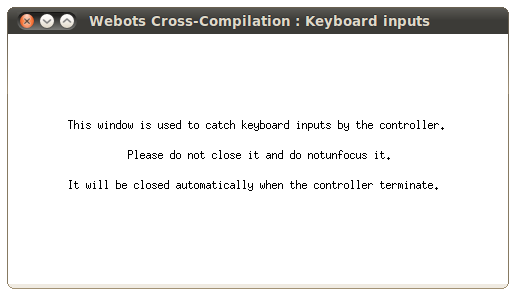
\includegraphics[width=10cm]{keyboardWindow.png}
\caption{Small window used to capture the keyboard inputs in cross-compilation.}
\label{keyboardWindow}
\end{center}
\end{figure}

This little window is used to capture the input of the keyboard. Please do not close this window or unset the focus on it (by clicking outside this window) or you wont be able to read the keyboard input anymore.\\

%%%%%%%%%%%%%%%%%%%%%%%%%%%%%%%%%%%%%%%%%%%%%%%%%%%%%%%%%%%%%%%%%%%%%%%%%%%%%%%%%

\newpage
\section{Remote control}

Remote-control, is much more simpler to use than cross-compilation, you do not have to set the time step in any files, or to edit any specific makefile, the exact same controller that in simulation can be used for remote control (without even having to recompile it). Moreover, the remote-control mode allows you to visualize the state of the sensors and actuators of the real robot in real time. To use remote-control, open the robot window, go to the \textit{Transfer} tab, as for cross-compilation you have to set the connection settings (the settings been the same as for cross-compilation, see previous chapter for more information). To start the remote control, stop and revert your simulation, put your robot in the stable position (see figure \ref{start_position}). Then press the following button:\\

\begin{figure}[H]
\begin{center}

\includegraphics[width=2.5cm]{remote.png}
\label{send}
\end{center}
\end{figure}

A small window (similar of the one from picture \ref{waitWindow}) will appear and ask you to wait until the remote-control has been started. When this window disappears and the eyes of the robot switch from red to green, the remote-control has been sucessfully started. You can now easily start and stop your controller in remote-control mode by using the run and stop button of Webots (see chapter \textit{Examples} for more details). Warning: if you revert the simulation it will stop the remote-control mode. In order to stop the remote-control (without reverting) simply press the stop button of the remote control (it has the same aspect from the one of the cross-compilation in figure \ref{stop}).\\

\begin{figure}[H]
\begin{center}
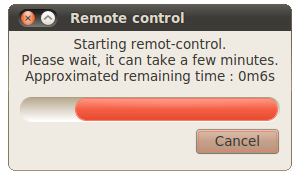
\includegraphics[width=6cm]{waitWindow.png}
\caption{This small window asks you to wait until remote-control has started.}
\label{waitWindow}
\end{center}
\end{figure}

When the controller runs in remote-control mode, you can see in the other tabs of the robot window the values of the sensors of the real robot in real-time.\\

\newpage
\subsection{Camera resolution}

In remote control, the camera's resolutions supported are not the same as in cross-compilation, indeed they are smaller in order to not slow down too much the communication speed between Webots and the robot. All the resolutions available are specified in table \ref{tab:cameraRemoteResolution}. Unlike from cross-compilation you do not have to specify the desired resolution in any file, the resolution is automatically send to the robot from Webots. So in order to adjust the resolution, just do the same way you would do it in the simulation (by editing \textit{cameraWidth} and \textit{cameraHeight} fields of the DARwIn-OP in the scene tree window).\\

\begin{table}[H]
\begin{center}
\begin{tabular}{| c | p{1cm} | c | }
\cline{1-1} \cline{3-3}
Width [pixel] &   & Height [pixel]\\ 
\cline{1-1} \cline{3-3}
\cline{1-1} \cline{3-3}
 320 &   & 240 \\
\cline{1-1} \cline{3-3}
160 &  & 120 \\
\cline{1-1} \cline{3-3}
80 &  & 80 \\
\cline{1-1} \cline{3-3}
40 &  & 60 \\
\cline{1-1} \cline{3-3}
20 &  & 40 \\
\cline{1-1}  \cline{3-3}
\multicolumn{1}{l}{}  &  & 30 \\
\cline{3-3}
\end{tabular}
\caption{Camera resolutions supported in remote-control.}
\label{tab:cameraRemoteResolution}
\end{center}
\end{table}

Note that you do not need to choose a width and a height from the same line, any combination of height and width is valid (for example, you can use a resolution of 320x30).\\

\subsection{Controller speed}
Your controller is supposed to run at a speed of 1.0x whatever you chose to run the simulation at run in \textit{real-time} or \textit{as fast as possible} mode. It can still happen sometimes that the speed can not achieve a speed of 1.0x, especialy when using the camera at high resolution, the mode \textit{as fast as possible without graphics} should resolve this problem.\\

If despite this you can not achieve a speed of 1.0x, it means that your connection with the robot is to slow. You should consider reducing camera resolution in order to increase the speed.\\

%%%%%%%%%%%%%%%%%%%%%%%%%%%%%%%%%%%%%%%%%%%%%%%%%%%%%%%%%%%%%%%%%%%%%%%%%%%%%%%%%

\newpage
\section{Known Bugs}

\subsection{Lateral balance}
In simulation, in the DARwInOPGaitManager, the lateral balance does not work as expected. It is recommended to set \textit{balance\_hip\_roll\_gain} and \textit{balance\_ankle\_roll\_gain} to 0.0, this must be done in the 'config.ini' file associated with the controller.\\

\subsection{Controller P}
In simulation the P gain of the servo affects the speed but on the real robot it affects the torque. This can cause differences between simulation and reality in some specific cases. Especially when P is small.\\

\subsection{Text-to-speech warning message}
When using one of the two functions of text to speech from the \textit{Speaker} module in cross-compilation, you might see the following message:
\begin{center}
bt\_audio\_service\_open : connect() failed : Connection refused (111)
\end{center}
You can simply ignore this message. This message is due to the fact that the robot is trying to communicate with a non-existent bluetooth device. You can supress this message by executing the following command on the robot:
\begin{center}
sudo apt-get purge bluez-alsa
\end{center}

%%%%%%%%%%%%%%%%%%%%%%%%%%%%%%%%%%%%%%%%%%%%%%%%%%%%%%%%%%%%%%%%%%%%%%%%%%%%%%%%%

\newpage
\section{Bibliography}

For any information about Webots, please visit Cyberbotics website: \url{http://www.cyberbotics.com}\\

Each time a new version of Webots is released the latest files of DARwIn-OP with Webots project are included, but you can always find the latest files of the project in the corresponding Github: \url{https://github.com/darwinop/webots-cross-compilation}\\

For any information about the DARwIn-OP robot please visit ROBOTIS website: \url{http://support.robotis.com/ko/product/darwin-op.htm}\\

DARwIn-OP being open source you can also find all the source files of the project here: \url{http://sourceforge.net/projects/darwinop}\\

%%%%%%%%%%%%%%%%%%%%%%%%%%%%%%%%%%%%%%%%%%%%%%%%%%%%%%%%%%%%%%%%%%%%%%%%%%%%%%%%%

\appendix
\newpage
\pagenumbering{Roman} %switch to roman enumeration

%%%%%%%%%%%%%%%%%%%%%%%%%%%%%%%%%%%%%%%%%%%%%%%%%%%%%%%%%%%%%%%%%%%%%%%%%%%%%%%%%

\section{Walking parameters} \label{sec:walkParameter}

This appendix explains all the parameters that can be set in the configuration file (.ini) to tune the gait.\\ 

\paragraph*{X offset}
is the offset of the feet in the X direction. Unit is in millimeter.
\begin{figure}[H]
\begin{center}
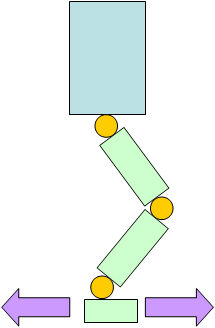
\includegraphics[width=3cm]{x_offset.jpg}
\caption{Walking : x offset parameters}
\label{x_offset}
\end{center}
\end{figure}

\paragraph*{Y offset}
is the offset of the feet in the Y direction. Unit is in millimeter.
\begin{figure}[H]
\begin{center}
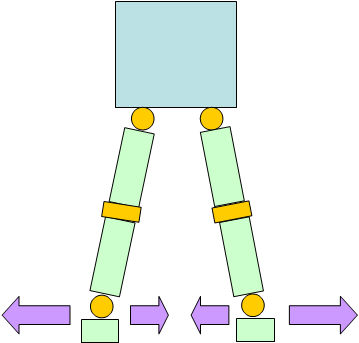
\includegraphics[height=6cm]{y_offset.jpg}
\caption{Walking : y offset parameters}
\label{y_offset}
\end{center}
\end{figure}

\newpage
\paragraph*{Z offset}
is the offset of the feet in the Z direction. Unit is in millimeter.
\begin{figure}[H]
\begin{center}
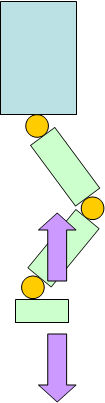
\includegraphics[height=6cm]{z_offset.jpg}
\caption{Walking : z offset parameters}
\label{z_offset}
\end{center}
\end{figure}

\paragraph*{Roll offset}
is the angle offset at the feet along X axis. Unit is in degree.
\begin{figure}[H]
\begin{center}
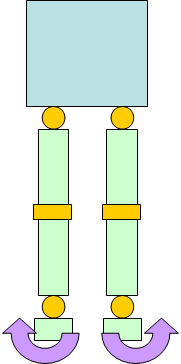
\includegraphics[height=6cm]{roll_offset.jpg}
\caption{Walking : roll offset parameters}
\label{roll_offset}
\end{center}
\end{figure}

\newpage
\paragraph*{Pitch offset}
is the angle offset at the feet along Y axis. Unit is in degree.
\begin{figure}[H]
\begin{center}
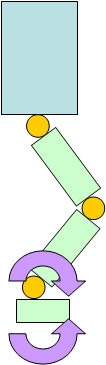
\includegraphics[height=6cm]{pitch_offset.jpg}
\caption{Walking : pitch offset parameters}
\label{pitch_offset}
\end{center}
\end{figure}

\paragraph*{Yaw offset}
is the angle offset of the leg along Z axis. Unit is in degree.
\begin{figure}[H]
\begin{center}
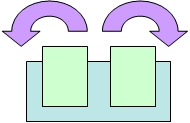
\includegraphics[height=2.5cm]{yaw_offset.jpg}
\caption{Walking : yaw offset parameters}
\label{yaw_offset}
\end{center}
\end{figure}

\paragraph*{Hip pitch offset}
is the tilt of DARwIn-OP's body. It uses a special unit of the motor correspondig to 2.85 degree.
\begin{figure}[H]
\begin{center}
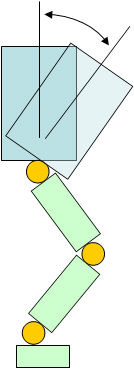
\includegraphics[height=6cm]{hip_pitch_offset.jpg}
\caption{Walking : hip pitch offset parameters}
\label{hip_pitch_offset}
\end{center}
\end{figure}

\newpage
\paragraph*{Period time}
is the time required for DArwIn-Op to complete two full steps (left and right foot). Unit is in millisecond.
\begin{figure}[H]
\begin{center}
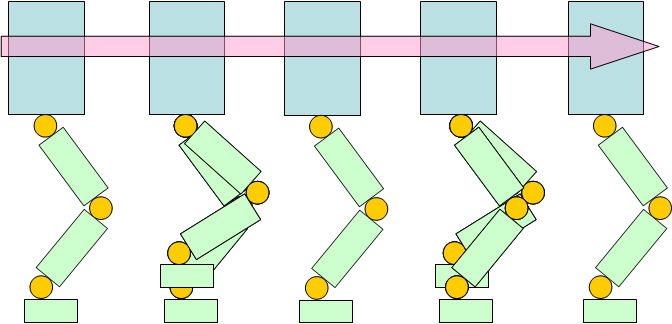
\includegraphics[width=8cm]{period_time.jpg}
\caption{Walking : period time parameters}
\label{period_time}
\end{center}
\end{figure}

\paragraph*{DSP ratio}
is the ratio between the time when both feet are on the ground to only one foot (either left or right) is on the ground.
\begin{figure}[H]
\begin{center}
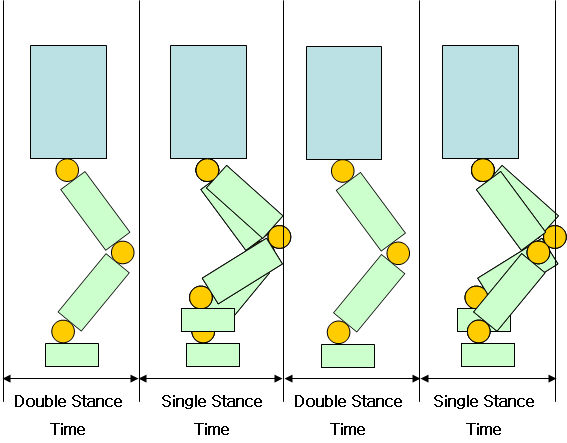
\includegraphics[width=8cm, height=5.5cm]{dsp_ratio.jpg}
\caption{Walking : dsp ratio parameters}
\label{dsp_ratio}
\end{center}
\end{figure}

\newpage
\paragraph*{Step forward back ratio}
is the differential distance according to X direction, between DARwIn-OP's left and right foot during walk. Unit is in millimeter.
\begin{figure}[H]
\begin{center}
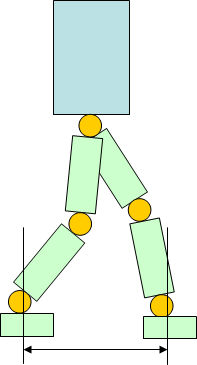
\includegraphics[height=4.5cm]{step_forward_back_ratio.jpg}
\caption{Walking : step forward back ratio parameters}
\label{step_forward_back_ratio}
\end{center}
\end{figure}

\paragraph*{Foot height}
is the maximum height of the foot during the step. Unit is in millimeter.
\begin{figure}[H]
\begin{center}
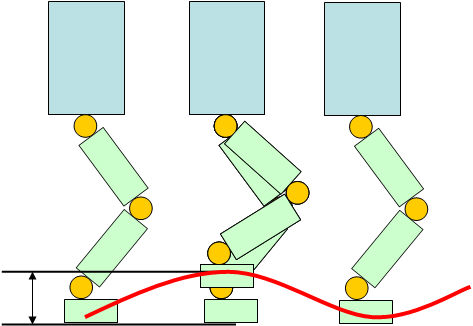
\includegraphics[height=4.5cm]{foot_height.jpg}
\caption{Walking : foot height parameters}
\label{foot_height}
\end{center}
\end{figure}

\paragraph*{Swing right left}
is the left and right Swaying of DARwIn-OP's body during walking. Unit is in millimeter.
\begin{figure}[H]
\begin{center}
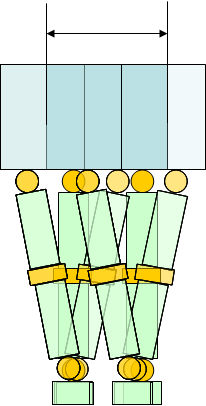
\includegraphics[height=6cm]{swing_right_left.jpg}
\caption{Walking : swing right left parameters}
\label{swing_right_left}
\end{center}
\end{figure}

\paragraph*{Swing top down}
is the up and down swaying of DARwIn-OP's body during walking. Unit is in millimeter.
\begin{figure}[H]
\begin{center}
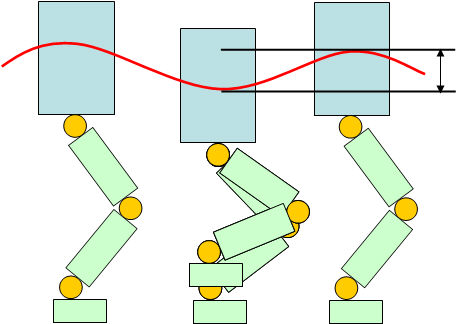
\includegraphics[height=5cm, width=8.5cm]{swing_top_down.jpg}
\caption{Walking : swing top down parameters}
\label{swing_top_down}
\end{center}
\end{figure}

\paragraph*{Pelvis offset}
is angle offset at the pelvis along X axis. It uses a special unit of the motor correspondig to 2.85 degree.
\begin{figure}[H]
\begin{center}
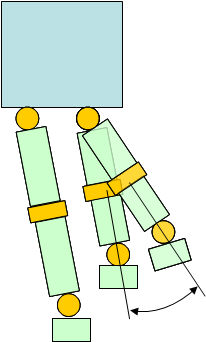
\includegraphics[height=5cm, width=3.7cm]{pelvis_offset.jpg}
\caption{Walking : pelvis offset parameters}
\label{pelvis_offset}
\end{center}
\end{figure}

\paragraph*{Arm swing gain}
is the gain that influences the movement of the arm during walking.

\paragraph*{Balance knee gain}
is the gain at the knee level for the front/back balance

\paragraph*{Balance ankle pitch gain}
is the gain at the ankle level for the front/back balance.

\paragraph*{Balance hip roll gain}
is the gain at the hip level for the lateral balance. Since the lateral balance does not work very well in simulation, we recommend you to set this parameter to 0.

\paragraph*{Balance ankle roll gain}
is the gain at the ankle level for the lateral balance. Since the lateral balance does not work very well in simulation, we recommend you to set this parameter to 0.


%%%%%%%%%%%%%%%%%%%%%%%%%%%%%%%%%%%%%%%%%%%%%%%%%%%%%%%%%%%%%%%%%%%%%%%%%%%%%%%%%

\section{Motions files} \label{sec:Motions}

\begin{table}[H]
\begin{center}
\begin{tabular}{ | c | c | c | c | }

\hline
ID & Name & Description & Recommended initial position \\ 
\hline
\hline
1 & ini & Move to standing position & Standing up \\
\hline
2 & OK & Nods head & Standing up \\
\hline
3 & no & Shakes head & Standing up \\
\hline
4 & hi & Tilts forward & Standing up \\
\hline
6 & talk1 & Holds out his hand & Standing up \\
\hline
9 & walkready & Prepares to walk & Standing up \\
\hline
10 & f up & Gets up & Lying face against the ground \\
\hline
11 & b up & Gets up & Lying back on the ground \\
\hline
12 & rk & Right shoot & Standing up \\
\hline
13 & lk & Left shoot & Standing up \\
\hline
15 & sit down & Sits & Standing up \\
\hline
16 & stand up & Stands up & Seated \\
\hline
17 & mul1 & Gets balanced on the head & Standing up \\
\hline
23 & d1 & Does yes with the arm & Standing up \\
\hline
24 & d2 & Applaud & Standing up \\
\hline
27 & d3 & Does yes with the arm and head & Standing up \\
\hline
29 & talk2 & Holds out his hand & Standing up \\
\hline
31 & d4 & Stretches in front and rear & Standing up \\
\hline
38 & d2 & Wave with the hand & Standing up \\
\hline
41 & talk2 & Presents himself & Standing up \\
\hline
54 & int & Applaud louder & Standing up \\
\hline
57 & int & Applaud & Standing up \\
\hline
70 & rPASS & Performs a pass with the right foot & Standing up \\
\hline
71 & lPASS & Performs a pass with the left foot & Standing up \\
\hline
90 & lie down & Lies on the front & Standing up \\
\hline
91 & lie up & Lies on the back & Standing up \\
\hline
237 & sitdown & Jumps up and down & Standing up \\
\hline
239 & sitdown & Jumps up and down quickly & Standing up \\
\hline
\end{tabular}
\caption{Motions stored in the motions files.}
\label{tab::Motions}
\end{center}
\end{table}

%%%%%%%%%%%%%%%%%%%%%%%%%%%%%%%%%%%%%%%%%%%%%%%%%%%%%%%%%%%%%%%%%%%%%%%%%%%%%%%%%

\section{Audio files available} \label{sec:audioFile}

\begin{table}[H]
\begin{center}
\begin{tabular}{ | c | c | c |  }

\hline
File & Lenght [sec] & Size [kB] \\ 
\hline
\hline
Autonomous soccer mode.mp3 & 1 & 29 \\
\hline
Bye bye.mp3 & 1 & 18.4 \\
\hline
Clap please.mp3 & 1 & 20.4 \\
\hline
Demonstration ready mode.mp3 & 2 & 31.5 \\
\hline
Headstand.mp3 & 1 & 19.2 \\
\hline
Interactive motion mode.mp3 & 1 & 29.8 \\
\hline
Introduction.mp3 & 16 & 258.8 \\
\hline
Left kick.mp3 & 1 & 17.2 \\
\hline
No.mp3 & 1 & 13.5 \\
\hline
Oops.mp3 & 1 & 14.7 \\
\hline
Right kick.mp3 & 1 & 18.4 \\
\hline
Sensor calibration complete.mp3 & 2 & 36.4 \\
\hline
Sensor calibration fail.mp3 & 2 & 37.2 \\
\hline
Shoot.mp3 & 1 & 15.5 \\
\hline
Sit down.mp3 & 1 & 20.4 \\
\hline
Stand up.mp3 & 1 & 19.6 \\
\hline
Start motion demonstration.mp3 & 2 & 34.3 \\
\hline
Start soccer demonstration.mp3 & 2 & 34.3 \\
\hline
Start vision processing demonstration.mp3 & 2 & 42.9 \\
\hline
System shutdown.mp3 & 1 & 26.2 \\
\hline
Thank you.mp3 & 1 & 17.2 \\
\hline
Vision processing mode.mp3 & 1 & 28.2 \\
\hline
Wow.mp3 & 1 & 17.6 \\
\hline
Yes.mp3 & 1 & 16.8 \\
\hline
Yes go.mp3 & 1 & 24.1 \\
\hline
\end{tabular}
\caption{Audio files already available on the robot in the directory /darwin/Data/mp3/}
\label{tab::audioFile}
\end{center}
\end{table}

%%%%%%%%%%%%%%%%%%%%%%%%%%%%%%%%%%%%%%%%%%%%%%%%%%%%%%%%%%%%%%%%%%%%%%%%%%%%%%%%%

\section{Voices available} \label{sec:voices}

\begin{table}[H]
\begin{center}
\begin{tabular}{ | c | c | | c | c |}
\hline
Name & Voice & Name & Voice \\ 
\hline
\hline
af & afrikaans & bs & bosnian \\
\hline
ca & catalan & cs & czech \\
\hline
cy & welsh & da & danish \\
\hline
de & german & el & greek \\
\hline
en & english & eo & esperanto \\
\hline
es & esperanto & fi & finnish \\
\hline
fr & french & grc & greek \\
\hline
hi & hindi & hr & croatian \\
\hline
hu & hungarian & hy & armenian \\
\hline
id & indonesian & is & icelandic \\
\hline
it & italian & ku & kurdish \\
\hline
la & latin & lv & latvian \\
\hline
mk & macedonian & nl & dutch \\
\hline
no & norwegian & pl & polish \\
\hline
pt & brazil & pt-pt & portugal \\
\hline
ro & romanian & ru & russian \\
\hline
sk & slovak & sq & albanian \\
\hline
sr & serbian & sv & swedish \\
\hline
sw & swahihi & ta & tamil \\
\hline
tr & turkish & vi & vietnam \\
\hline
zh & Mandarin & & \\
\hline
\end{tabular}
\caption{Available audio voices}
\label{tab::voices}
\end{center}
\end{table}

%%%%%%%%%%%%%%%%%%%%%%%%%%%%%%%%%%%%%%%%%%%%%%%%%%%%%%%%%%%%%%%%%%%%%%%%%%%%%%%%%

\end{document}
